\documentclass[a4paper,12pt]{article}
\usepackage[top=2cm,bottom=2cm,left=2.5cm,right=1.5cm]{geometry}
\usepackage{fontspec}
\usepackage{polyglossia}
\setmainlanguage{russian}
\IfFontExistsTF{Times New Roman}{%
  \setmainfont{Times New Roman}[Ligatures=TeX]%
  \newfontfamily\cyrillicfont{Times New Roman}[Ligatures=TeX]%
}{\IfFontExistsTF{CMU Serif}{%
  \setmainfont{CMU Serif}[Ligatures=TeX]%
  \newfontfamily\cyrillicfont{CMU Serif}[Ligatures=TeX]%
}{}}
\IfFontExistsTF{Courier New}{%
  \setmonofont{Courier New}%
  \newfontfamily\cyrillicfonttt{Courier New}%
}{\IfFontExistsTF{CMU Typewriter Text}{%
  \setmonofont{CMU Typewriter Text}%
  \newfontfamily\cyrillicfonttt{CMU Typewriter Text}%
}{}}
\usepackage{amsmath,amssymb}
\usepackage{float}
\usepackage{graphicx}
\usepackage{array}
\usepackage{setspace}
\setstretch{1.1}
\setlength{\parindent}{0pt}
\setlength{\parskip}{4pt}
\renewcommand{\arraystretch}{1.25}
\setlength{\tabcolsep}{4.5pt}

\begin{document}

\begin{center}
{\large\bfseries Лабораторная работа\\[2pt]
Поиск глобального минимума липшицевой функции методом ломаных (метод Пиявского)}\\[4pt]
Дисциплина: Методы оптимизации
\end{center}

\begin{tabular}{@{}ll}
Ф.И.О.: & Артемов Илья Витальевич\\
Поток: & 1.1\\
Вариант задания: & 1\\
\end{tabular}

\section{Постановка задачи}

Найти приближённо глобальный минимум функции одной переменной $f(x)$ на отрезке $[a,b]$ с точностью $\varepsilon$. Функция липшицева: существует такая константа $L > 0$, что $|f(x) - f(y)| \le L\,|x - y|$ для всех $x, y \in [a,b]$.

Программа на Python принимает строку с функцией (например, $f(x) = x + \sin(3{,}14159\,x)$), концы отрезка $a$, $b$ и точность $\varepsilon$. Она выводит график функции, вспомогательные функции (ломаные, в том числе итоговую, на которой достигнута требуемая точность), приближённые значения аргумента $x^*$ и минимума $f(x^*)$, число итераций и затраченное время.

\textbf{Тестовая функция.} Работа программы показана на одномерном срезе ($y = 0$) двумерной функции Растригина. Отрезок $[-3;\,4]$ выбран несимметричным, точность $\varepsilon = 0{,}01$.
\[
f(x,y) = 20 + x^2 + y^2 - 10\cos 2\pi x - 10\cos 2\pi y,
\qquad
f(x) = f(x,0) = 10 + x^2 - 10\cos 2\pi x.
\]
На отрезке $[-3;\,4]$ у функции 8 локальных минимумов.

\textbf{Обозначения, по которым ведётся расчёт.}
\begin{itemize}
\item $x_1 < x_2 < \dots < x_n$ - точки, в которых уже вычислена функция (испытания), $f_i = f(x_i)$; $f^*_n = \min_i f_i$ - лучшее найденное значение, $x^*$ - точка, где оно достигнуто.
\item $F_n(x)$ - вспомогательная функция (ломаная), построенная по $n$ испытаниям; всегда $F_n \le f$.
\item $v_i$ и $R_i$ - абсцисса и значение нижнего излома ломаной на отрезке $[x_i, x_{i+1}]$; $m_n = \min_i R_i$ - наименьшее значение ломаной.
\item Итерация - одно новое испытание. Число итераций равно $N - 2$, где $N$ - общее число вычислений $f$ (два начальных испытания в концах отрезка и все последующие).
\end{itemize}

\section{Ход решения}

\subsection*{Шаг 1. Нижняя оценка функции: ломаная}

Из условия Липшица для любого испытания $x_i$ и любой точки $x \in [a,b]$ следует $f(x) \ge f_i - L\,|x - x_i|$. Поэтому
\[
f(x) \ \ge\ F_n(x) = \max_{1 \le i \le n}\bigl(f_i - L\,|x - x_i|\bigr).
\]
График $F_n$ - ломаная: в точках $x_i$ она касается графика $f$ ($F_n(x_i) = f_i$), а между соседними испытаниями имеет излом вниз. Чем больше испытаний, тем теснее ломаная прижимается к $f$ (рис.~\ref{fig:rastrigin}).

На отрезке $[x_i, x_{i+1}]$ ломаная - максимум двух прямых $y = f_i - L(x - x_i)$ и $y = f_{i+1} + L(x - x_{i+1})$. Приравняв их, находим нижний излом:
\[
v_i = \frac{x_i + x_{i+1}}{2} + \frac{f_i - f_{i+1}}{2L},
\qquad
R_i = \frac{f_i + f_{i+1}}{2} - \frac{L\,(x_{i+1} - x_i)}{2}.
\]

\subsection*{Шаг 2. Точность и алгоритм}

Так как $F_n \le f$ на всём отрезке, то $m_n = \min F_n \le \min f$. С другой стороны, $\min f \le f^*_n$. Значит,
\[
m_n \ \le\ \min_{[a,b]} f \ \le\ f^*_n,
\]
и если $f^*_n - m_n \le \varepsilon$, то $f^*_n - \min f \le \varepsilon$: найденное значение отличается от глобального минимума не более чем на $\varepsilon$. Это условие остановки.

Алгоритм:
\begin{enumerate}
\item Взять $x_1 = a$, $x_2 = b$, вычислить $f_1$, $f_2$; $f^* = \min(f_1, f_2)$.
\item Для каждого интервала $[x_i, x_{i+1}]$ вычислить $v_i$ и $R_i$. Выбрать интервал с наименьшим $R_i$ (при равенстве - левый).
\item Выполнить испытание в точке $v_i$ выбранного интервала, вычислить $f(v_i)$, при необходимости обновить $f^*$ и $x^*$. Интервал делится на два.
\item Найти новое $m = \min R_i$. Если $f^* - m \le \varepsilon$, остановиться: ответ $x^*$, $f^*$. Иначе перейти к пункту 2.
\end{enumerate}

\subsection*{Шаг 3. Константа Липшица}

На вход программы константа $L$ не подаётся, поэтому программа оценивает её сама: вычисляет $f$ в $200001$ равноотстоящих узлах отрезка и берёт наибольший модуль разностных отношений $|f(x_{j+1}) - f(x_j)|/(x_{j+1} - x_j)$.

\subsection*{Шаг 4. Программа}

Программа \texttt{piyavsky.py} реализует алгоритм шага 2. В строке с функцией допустимы переменная \texttt{x}, арифметика, степень (\texttt{**} или \texttt{\^{}}), функции \texttt{sin}, \texttt{cos}, \texttt{tan}, \texttt{atan}, \texttt{sinh}, \texttt{cosh}, \texttt{tanh}, \texttt{exp}, \texttt{log}, \texttt{sqrt}, \texttt{abs} и константы \texttt{pi}, \texttt{e}.

Программа запрашивает с клавиатуры функцию, концы отрезка $a$, $b$ и точность $\varepsilon$ (десятичный разделитель - точка или запятая). Ввод для тестовой функции:

\begin{minipage}{\textwidth}
\begin{verbatim}
python3 piyavsky.py
Функция f(x): f(x) = 10 + x^2 - 10*cos(2*pi*x)
Левый конец отрезка a: -3
Правый конец отрезка b: 4
Точность eps: 0.01
\end{verbatim}
\end{minipage}
\medskip

В консоль выводятся $L$, $x^*$, $f(x^*)$, нижняя оценка $m_N$, число итераций и время счёта (от оценки $L$ до конца итераций, без построения графика). На графике показаны: $f(x)$, итоговая ломаная, точки испытаний, найденный минимум (красная звезда) и ломаные после $4$, $10$ и $30$ испытаний (если испытаний было больше соответствующего числа).

\subsection*{Шаг 5. Первые итерации на функции Растригина}

Берём функцию Растригина на $[-3;\,4]$, $\varepsilon = 0{,}01$, $L = 69{,}3327$.

\textbf{Начало.} $x_1 = -3$, $x_2 = 4$: $f(-3) = 10 + 9 - 10\cos 6\pi = 9$, $f(4) = 10 + 16 - 10\cos 8\pi = 16$. $f^* = 9$ (в точке $x^* = -3$).

\textbf{Итерация 1.} Единственный интервал $[-3;\,4]$:
\begin{align*}
R_1 &= \frac{9 + 16}{2} - \frac{69{,}3327 \cdot 7}{2} = 12{,}5 - 242{,}6643 = -230{,}1643,\\
v_1 &= \frac{-3 + 4}{2} + \frac{9 - 16}{2 \cdot 69{,}3327} = 0{,}5 - 0{,}050481 = 0{,}449519.
\end{align*}
Испытание: $f(0{,}449519) = 10 + 0{,}449519^2 - 10\cos(2\pi \cdot 0{,}449519) = 19{,}7032$, рекорд не улучшился, $f^* = 9$. Интервал делится на $[-3;\,0{,}4495]$ и $[0{,}4495;\,4]$. Для обоих $R = -105{,}2305$ (в общем случае обе новые величины равны $(R_i + f(v_i))/2$; здесь $(-230{,}1643 + 19{,}7032)/2 = -105{,}2305$). Тогда $m = -105{,}2305$, $f^* - m = 114{,}2305 > \varepsilon$.

\textbf{Итерация 2.} Наименьшее $R$ у обоих интервалов одно и то же, берём левый $[-3;\,0{,}4495]$: $v = -1{,}3524$, $f(v) = 17{,}8297$. Новые $R$ у двух его половин равны $(-105{,}2305 + 17{,}8297)/2 = -43{,}7004$; правый интервал $[0{,}4495;\,4]$ по-прежнему имеет $R = -105{,}2305$, поэтому $m$ не изменилось.

Дальнейшие итерации считаются так же. В таблице~\ref{tab:trace} показаны первые шесть и последняя, 135-я итерация (значения округлены до четырёх знаков, $R$ - значение излома выбранного интервала, $m_{n+1}$ - наименьшее $R$ после испытания).

\begin{table}[H]
\centering\small
\caption{Функция Растригина, итерации метода ломаных}
\label{tab:trace}
\begin{tabular}{|c|c|r|r|r|r|r|r|}
\hline
$k$ & Интервал $[x_i;\,x_{i+1}]$ & $R$ & $v$ & $f(v)$ & $f^*$ & $m_{n+1}$ & $f^* - m_{n+1}$ \\ \hline
1 & $-3{,}0000;\ 4{,}0000$ & $-230{,}1643$ & $0{,}4495$ & $19{,}7032$ & $9$ & $-105{,}2305$ & $114{,}2305$ \\
2 & $-3{,}0000;\ 0{,}4495$ & $-105{,}2305$ & $-1{,}3524$ & $17{,}8297$ & $9$ & $-105{,}2305$ & $114{,}2305$ \\
3 & $0{,}4495;\ 4{,}0000$ & $-105{,}2305$ & $2{,}2515$ & $15{,}1612$ & $9$ & $-45{,}0347$ & $54{,}0347$ \\
4 & $0{,}4495;\ 2{,}2515$ & $-45{,}0347$ & $1{,}3832$ & $19{,}3412$ & $9$ & $-45{,}0347$ & $54{,}0347$ \\
5 & $2{,}2515;\ 4{,}0000$ & $-45{,}0347$ & $3{,}1197$ & $12{,}4291$ & $9$ & $-43{,}7004$ & $52{,}7004$ \\
6 & $-3{,}0000;\ -1{,}3524$ & $-43{,}7004$ & $-2{,}2399$ & $14{,}3823$ & $9$ & $-43{,}7004$ & $52{,}7004$ \\
\dots & \multicolumn{7}{c|}{\dots} \\
135 & $0{,}0049;\ 0{,}0054$ & $-0{,}0118$ & $0{,}0052$ & $0{,}0053$ & $2{,}3 \cdot 10^{-6}$ & $-0{,}0092$ & $0{,}0092$ \\
\hline
\end{tabular}
\end{table}

После 135-й итерации $f^* - m = 0{,}0092 \le 0{,}01$, условие остановки выполнено.

\subsection*{Шаг 6. Результаты для функции Растригина}

Вывод программы и график (рис.~\ref{fig:rastrigin}) для функции Растригина на $[-3;\,4]$, $\varepsilon = 0{,}01$:

\begin{figure}[H]
\centering
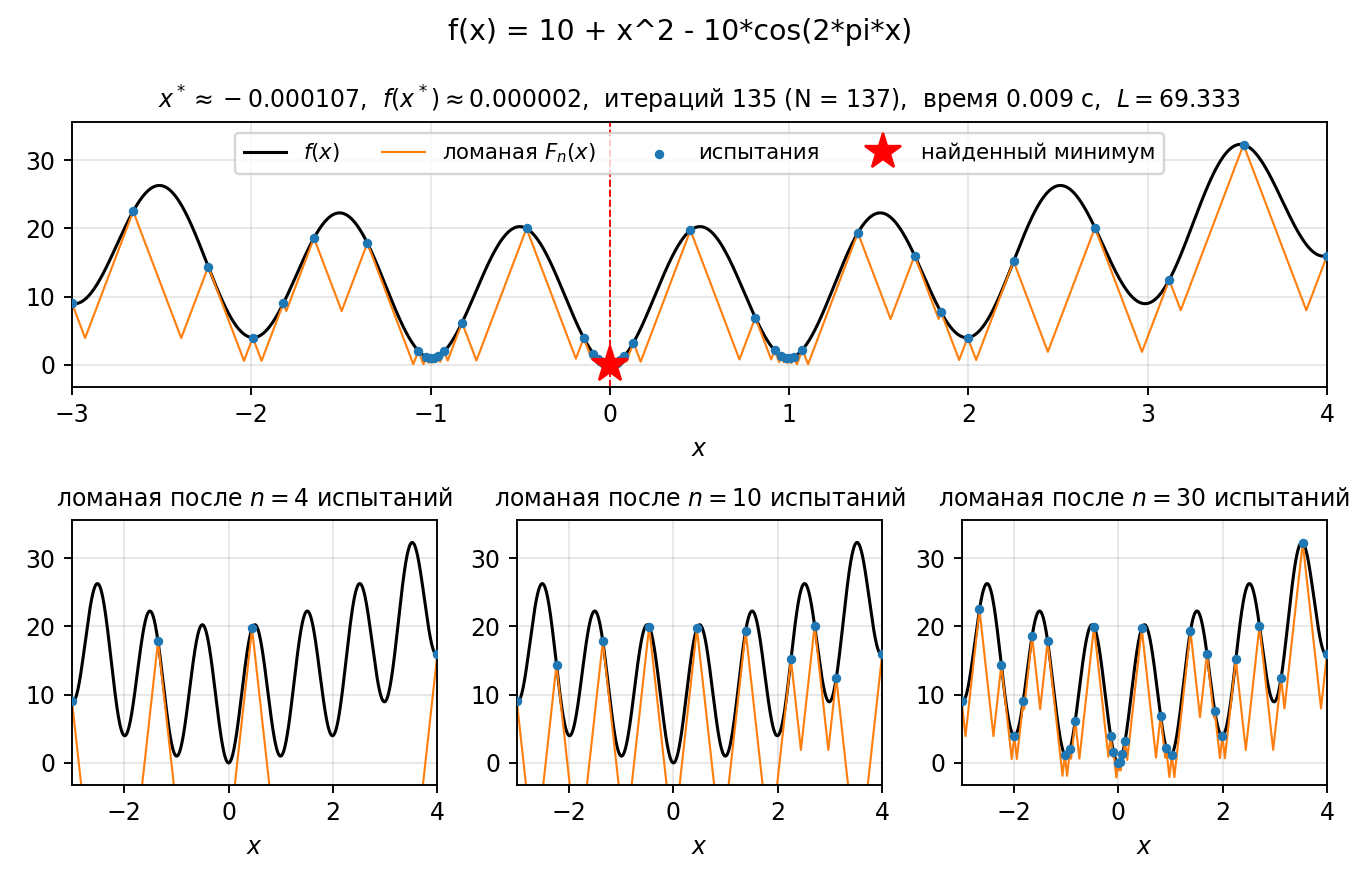
\includegraphics[width=0.92\textwidth]{screenshots/rastrigin.png}
\caption{Функция Растригина: график, итоговая ломаная, найденный минимум и ломаные после $4$, $10$, $30$ испытаний}
\label{fig:rastrigin}
\end{figure}

\begin{table}[H]
\centering
\caption{Функция Растригина, результат работы программы}
\begin{tabular}{|l|l|}
\hline
Константа Липшица (оценка) $L$ & $69{,}3327$\\ \hline
Приближённый аргумент минимума $x^*$ & $-0{,}000107$\\ \hline
Приближённое значение минимума $f(x^*)$ & $2{,}3 \cdot 10^{-6}$\\ \hline
Нижняя оценка минимума $m_N$ & $-0{,}009236$\\ \hline
Разность $f(x^*) - m_N$ & $0{,}009238 \le \varepsilon$\\ \hline
Число итераций & $135$ ($N = 137$ вычислений $f$)\\ \hline
Время счёта & $0{,}0089$ с (зависит от компьютера и запуска)\\ \hline
\end{tabular}
\end{table}

Больше всего испытаний сделано около глобального минимума $x = 0$, около локальных минимумов с большими значениями их мало: к моменту остановки все изломы ломаной лежат не ниже $m_N \ge f^* - \varepsilon$, то есть ни на одном интервале функция не может опуститься ниже $f^* - \varepsilon$.

\subsection*{Шаг 7. Ответ}

Приближённое решение задачи для тестовой функции (отрезок $[-3;\,4]$, $\varepsilon = 0{,}01$):
\[
x^* \approx -0{,}000107 \in [-3;\,4], \qquad f(x^*) \approx 2{,}3 \cdot 10^{-6}, \qquad 135 \text{ итераций}.
\]

\section{Рефлективный вывод}

\textbf{Что оказалось полезным.} Метод даёт приближённое решение, а также доказательство его точности: ломаная $F_n$ является нижней оценкой функции, и пока $f^*_n - m_n > \varepsilon$, остаются интервалы, где минимум может лежать ниже рекорда. Так стало понятно, что глобальный поиск отличается от локального тем, что он не спускается в один минимум, а отсекает области, где лучшего значения быть не может.

\textbf{Трудности и как они преодолевались.}
\begin{enumerate}
\item На вход программы не подаётся константа Липшица, а метод без неё неприменим. Поэтому программа оценивает $L$ сама по значениям функции на сетке из $200001$ узла (наибольшее разностное отношение), и так работает для любой введённой функции.
\item Отрезок для демонстрации нужно было выбрать удачно. На симметричном отрезке с концами $-5{,}12$ и $5{,}12$ для функции Растригина первая же точка испытания - середина $x = 0$, то есть сразу глобальный минимум, и демонстрация получается неинформативной. Поэтому я взял несимметричный отрезок $[-3;\,4]$.
\end{enumerate}

\end{document}
